\documentclass{abntex2}
\usepackage[utf8]{inputenc}
\usepackage{graphicx}
\usepackage[num]{abntex2cite}



\titulo{Experimento 6: Imperfeições CC e não-linearidades}
\autor{Lucas Rezende de Macedo - 14/0026363\\Jônatas Ribeiro Senna Pires - 14/0090983}
\data{4 de Junho de 2018}
\local{Brasília, Distrito Federal}

\begin{document}

\imprimircapa
\imprimirfolhaderosto

\tableofcontents
\clearpage
\listoffigures
\clearpage

\chapter{Experiências}

 O objetivo do presente experimento consiste na verificação das características peculiares presentes
 em amplificadores operacionais reais, características as quais não são ideiais.

\section{Experiência}
\subsection{Experiência 1}

Foi montado o circuito de acordo com a figura \ref{fig:circuito1}, obtendo, assim, a montagem da figura \ref{fig:montagem1}.
\begin{figure}[h]
  \centering
  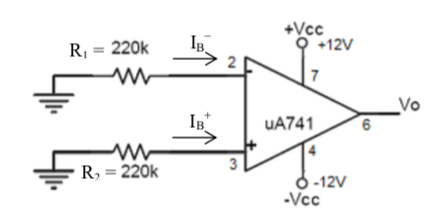
\includegraphics[scale = 0.5]{exp1.png}
  \caption{Circuito de caracterização da corrente de polarização de entrada e da corrente de compensação de entrada.}
  \label{fig:circuito1}
\end{figure}

Para este experimento, a mesma montagem foi realizada uma vez para cada um dos seguintes valores de $R_1$ e $R_2$ (medidos):
\begin{itemize}
  \item Montagem 1 - $R_1 = 197,8k\Omega$ e $R_2 = 202,3k\Omega$
  \item Montagem 2 - $R_1 = 98,9k\Omega$ e $R_2 = 98,3k\Omega$
  \item Montagem 3 - $R_1 = 99,9\Omega$ e $R_2 = 99,0\Omega$
\end{itemize}

\subsubsection{Parte 1 - Montagem}

\begin{figure}[h]
  \centering
  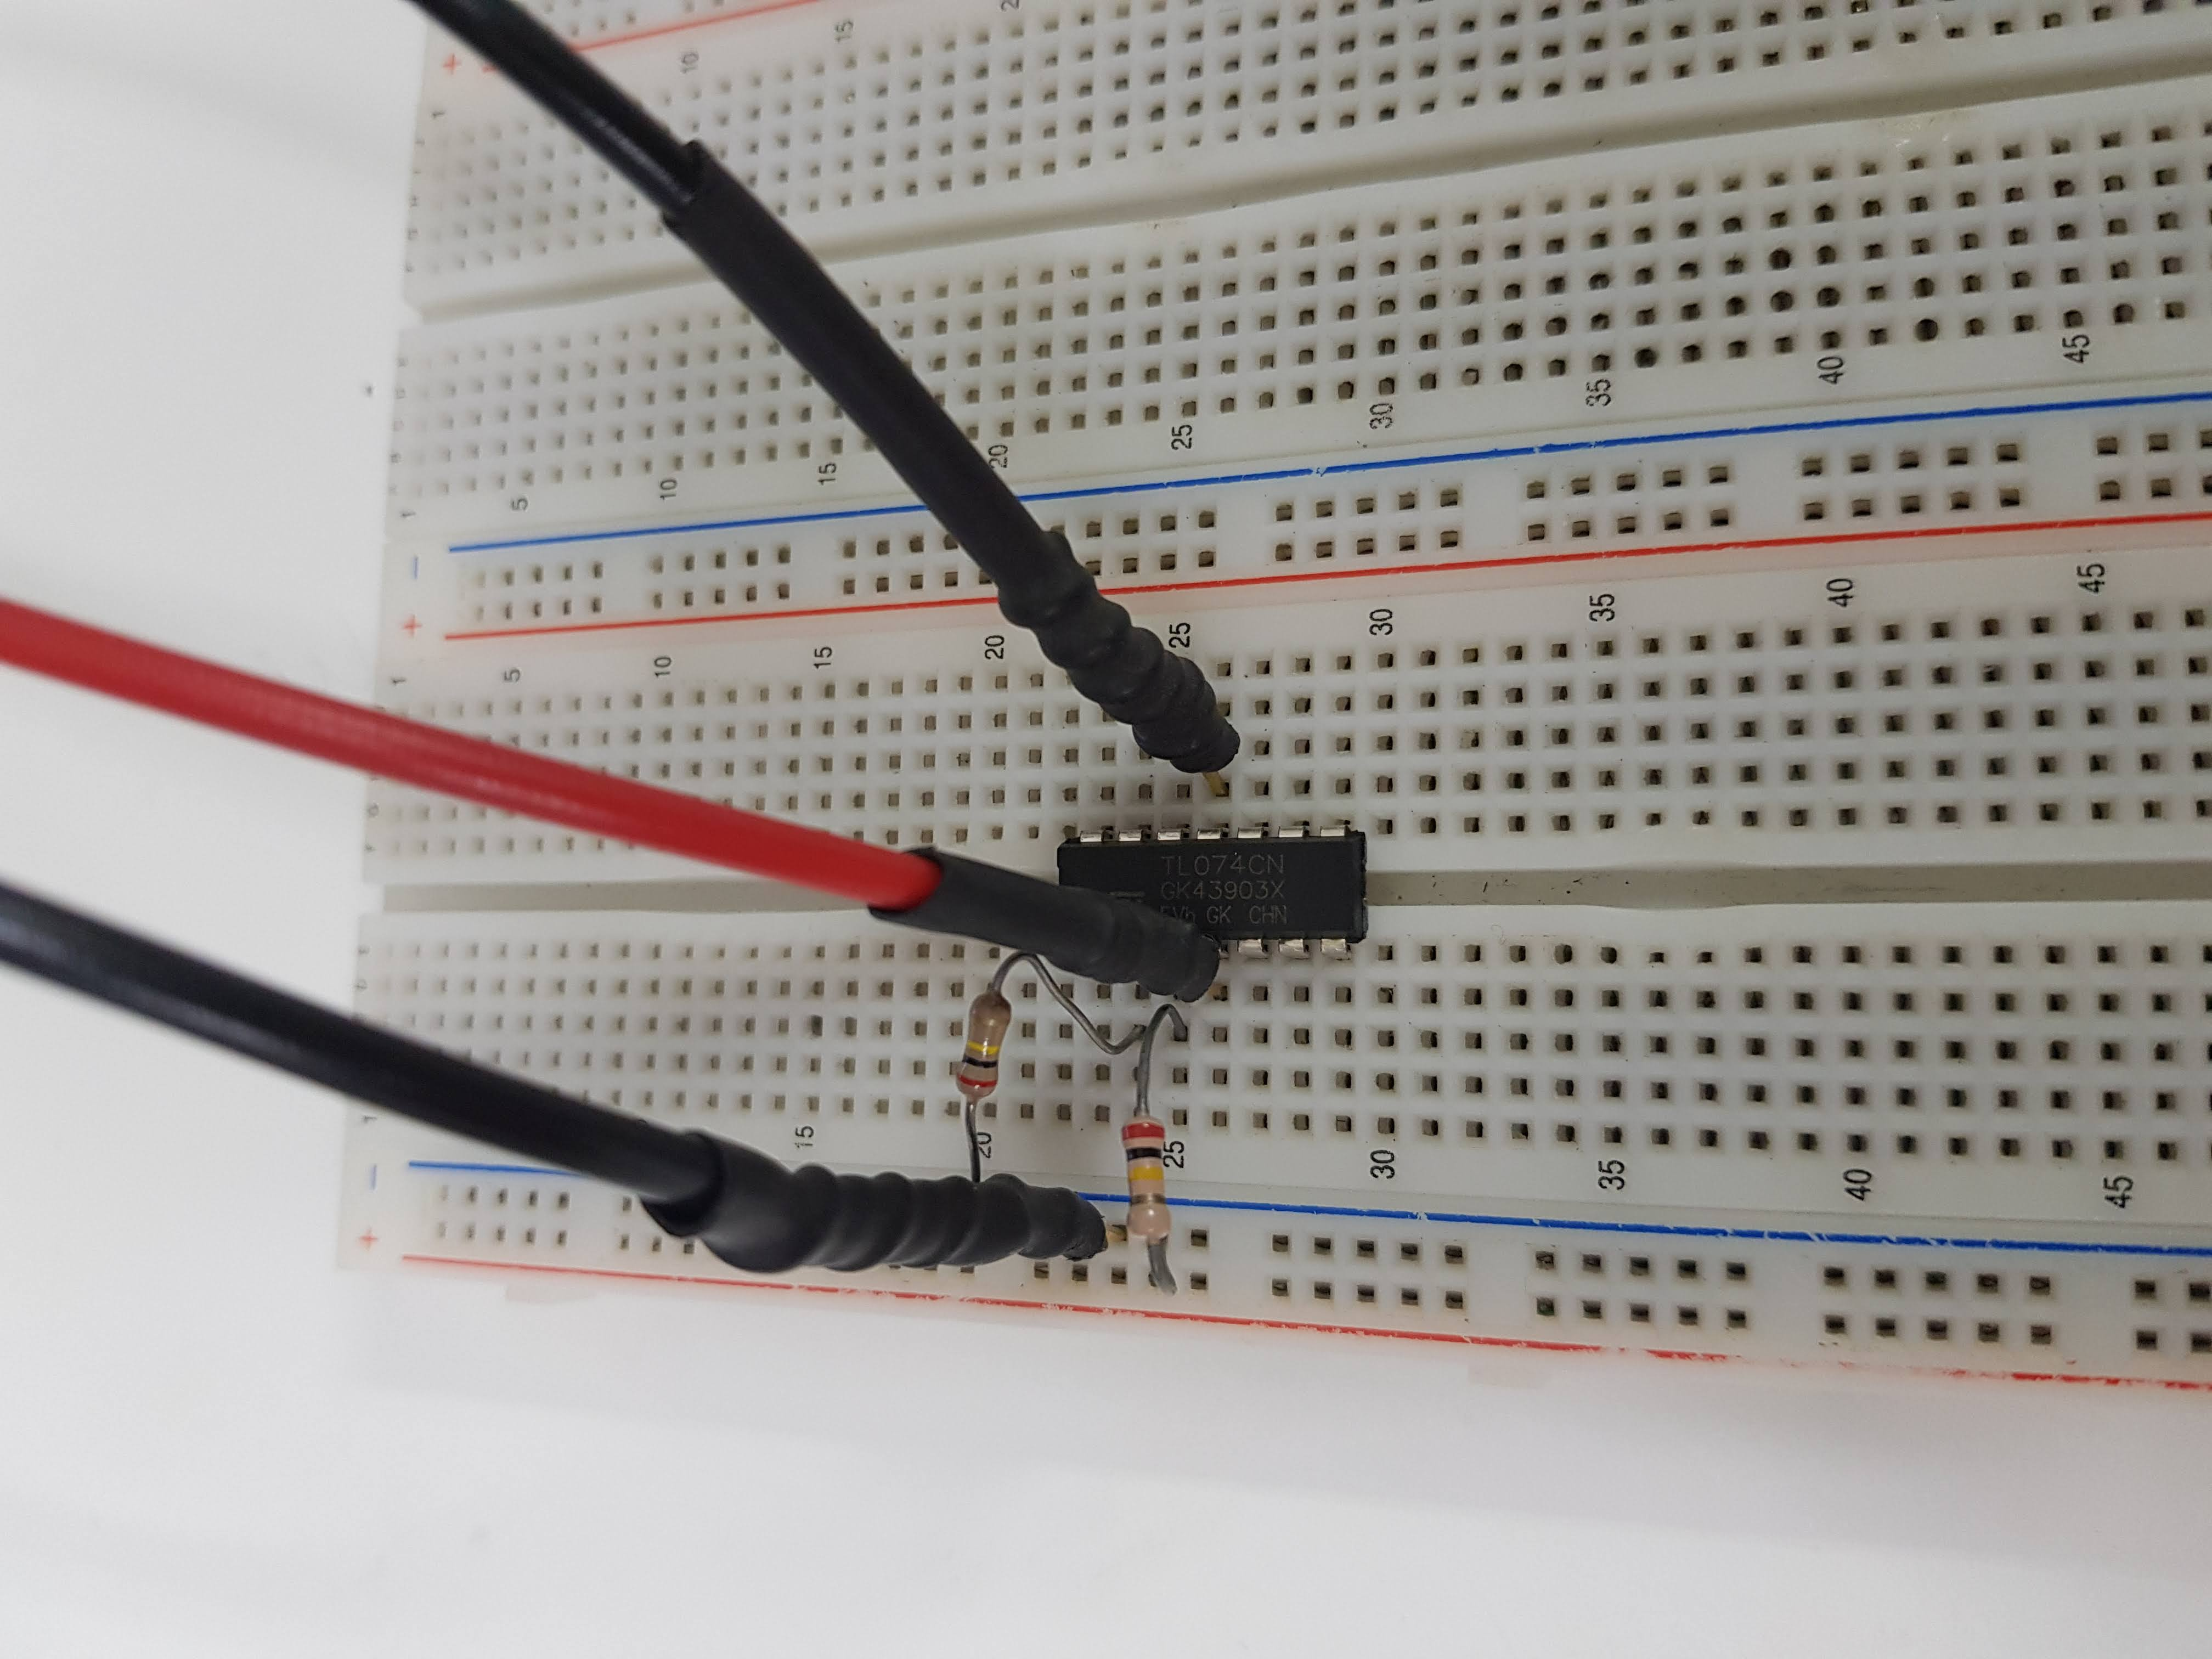
\includegraphics[scale = 0.5]{circ_0.png}
  \caption{Montagem do circuito da figura \ref{fig:circuito1}.}
  \label{fig:montagem1}
\end{figure}

\subsubsection{Parte 2}

  Foi medida a tensão DC nos terminais inversor e não-inversor, obtendo os seguintes valores para cada montagem:
  \begin{itemize}
    \item Montagem 1 - $V- = 1,7mV$ e $V+ = 1,7mV$
    \item Montagem 2 - $V- = 0,8mV$ e $V+ = 0,8mV$
    \item Montagem 3 - $V- = 0V$ e $V+ = 0V$
  \end{itemize}

\subsubsection{Parte 3}

  Utilizando a lei de Ohm e a fórmula fornecida no roteiro (\ref{eq:eq1}), foi calculada a corrente de compensação de entrada para cada montagem:
\begin{equation}
    $I_B = (I_B⁺ + I_B⁻)/2 $
  \label{eq:eq1}
\end{equation}

\begin{itemize}
  \item Montagem 1 - $I_B⁺ = 8,4nA$, $I_B⁻ = 8,59nA$ e $I_B = 8,5nA$
  \item Montagem 2 - $I_B⁺ = 8,14nA$, $I_B⁻ = 8,09nA$ e $I_B = 8,11nA$
  \item Montagem 3 - $I_B⁺ = 0A$, $I_B⁻ = 0A$ e $I_B = 0A$
\end{itemize}

\subsubsection{Parte 4}
  Foi calculada a a diferença entre correntes de compensação para a determinação da corrente de polarização para cada montagem:
  \begin{itemize}
    \item Montagem 1 - $I_O_S = -0,19nA$
    \item Montagem 2 - $I_O_S = 0,05nA$
    \item Montagem 3 - $I_O_S = 0A$
  \end{itemize}

\subsubsection{Parte 5}

Após a aquisição de todos os dados necessários, foi construída a seguinte tabela:

TABELAAAAAAAAA
\subsection{Experiência 2}

Foi montado o circuito de acordo com a figura \ref{fig:circuito2}, obtendo, assim, a montagem da figura \ref{fig:montagem2}.

\begin{figure}[h]
  \centering
  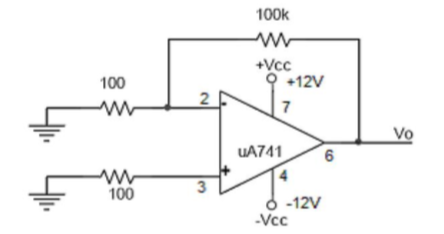
\includegraphics[scale = 0.5]{exp2.png}
  \caption{Circuito para medida das tensões de compensação de entrada e saída.}
  \label{fig:circuito2}
\end{figure}

Para este experimento, a mesma montagem foi realizada uma vez para cada um dos seguintes valores de R (medidos):
\begin{itemize}
  \item Montagem 1 - $R = 98,9k\Omega$
  \item Montagem 2 - $R = 202,3k\Omega$
  \item Montagem 3 - $R = 978\Omega$
\end{itemize}

\subsubsection{Parte 1 - Montagem}

\begin{figure}[h]
  \centering
  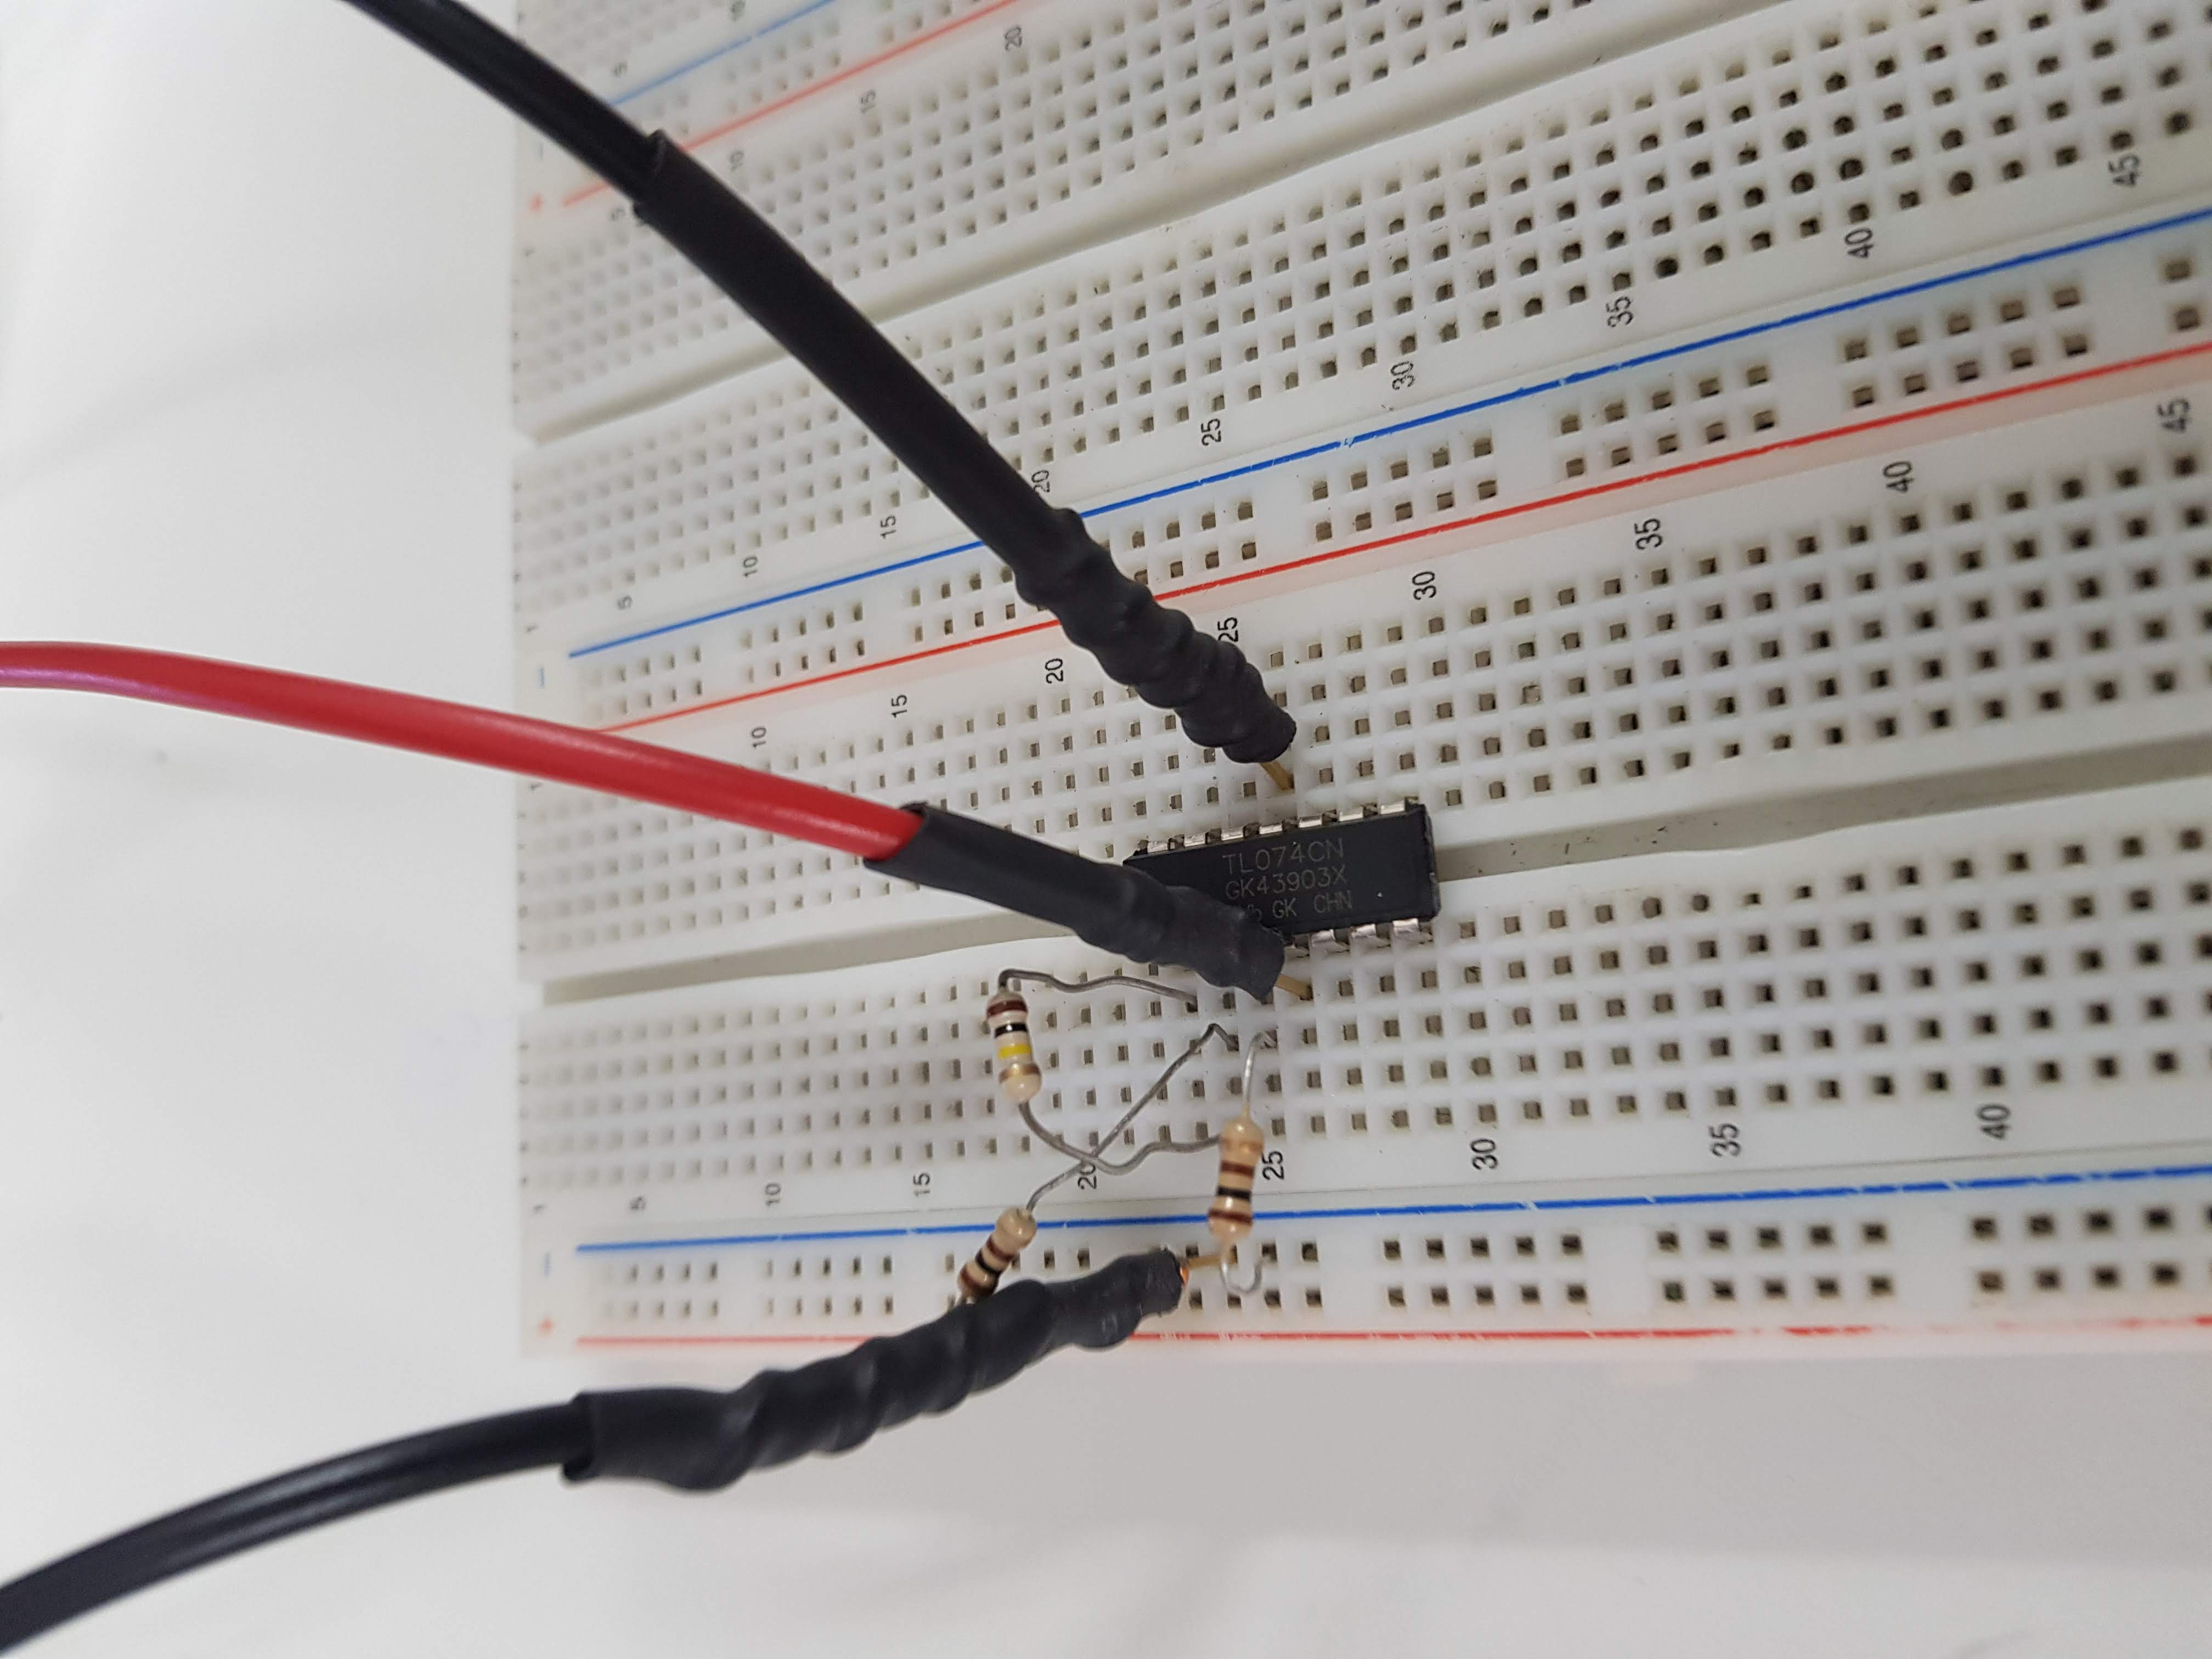
\includegraphics[scale = 0.5]{circ_1.png}
  \caption{Montagem do circuito da figura \ref{fig:circuito2}.}
  \label{fig:montagem2}
\end{figure}

\subsubsection{Parte 2}
Para cada montagem, foi medida a tensão DC de saída:
\begin{itemize}
  \item Montagem 1 - $V_o = -0,47V$
  \item Montagem 2 - $V_o = -0,95V$
  \item Montagem 3 - $V_o = -5,1mV$
\end{itemize}
\subsubsection{Parte 3}
Para cada montagem foi calculada a tensão de polarização de entrada:

\begin{itemize}
  \item Montagem 1 - $V_o_s = -0,47mV$
  \item Montagem 2 - $V_o_s = -0,47mV$
  \item Montagem 3 - $V_o_s = -0,47mV$
\end{itemize}

\subsubsection{Parte 4}
Após a aquisição dos dados necessários, foi construída a seguinte tabela:

TABELAAAAAAAAA

\subsection{Experiência 3}

Foram montados os circuitos de acordo com a figura \ref{fig:circuito3}, obtendo, assim, as montagens das figuras \ref{fig:montagem3} e \ref{fig:montagem4}.

\begin{figure}[h]
  \centering
  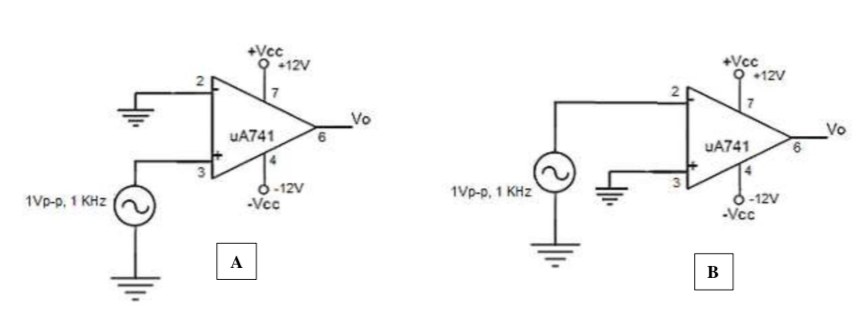
\includegraphics[scale = 0.5]{exp3.png}
  \caption{circuitos para medição das tensões de saturação.}
  \label{fig:circuito3}
\end{figure}

\subsubsection{Parte 1 - Montagem}

\begin{figure}[h]
  \centering
  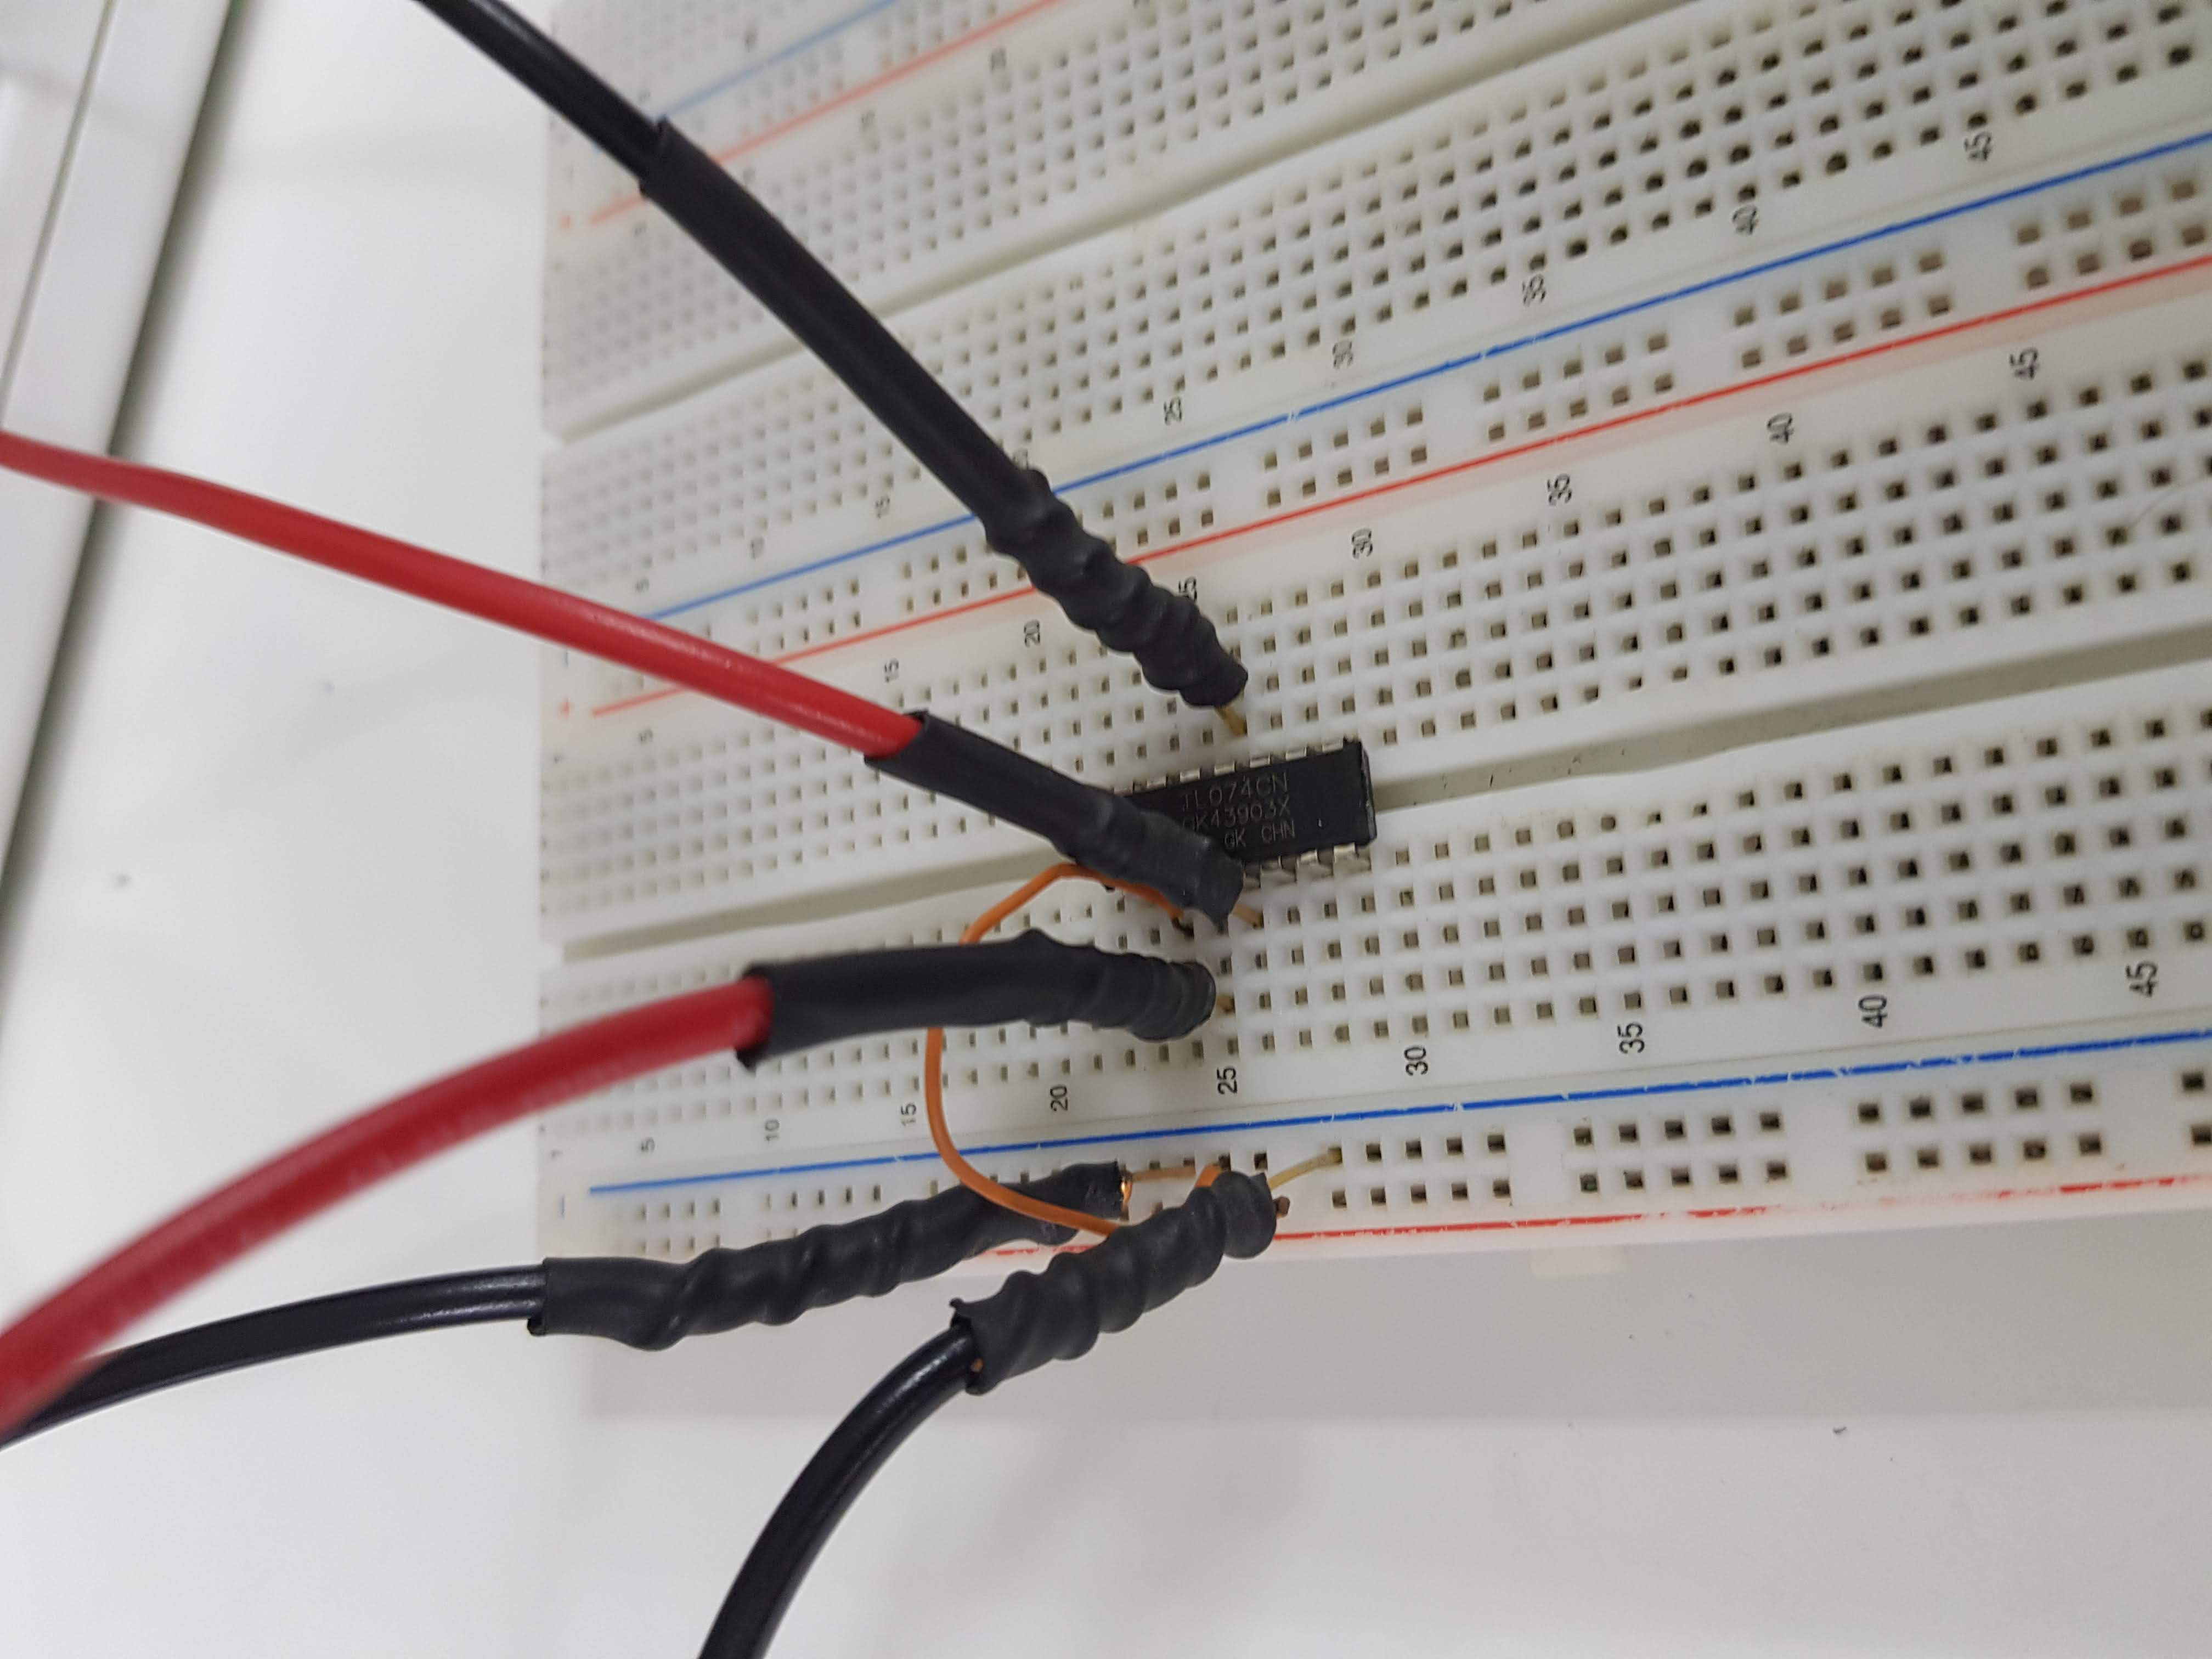
\includegraphics[scale = 0.5]{circ_2.png}
  \caption{Montagem do circuito da figura \ref{fig:circuito3} A.}
  \label{fig:montagem3}
\end{figure}
\begin{figure}[h]
  \centering
  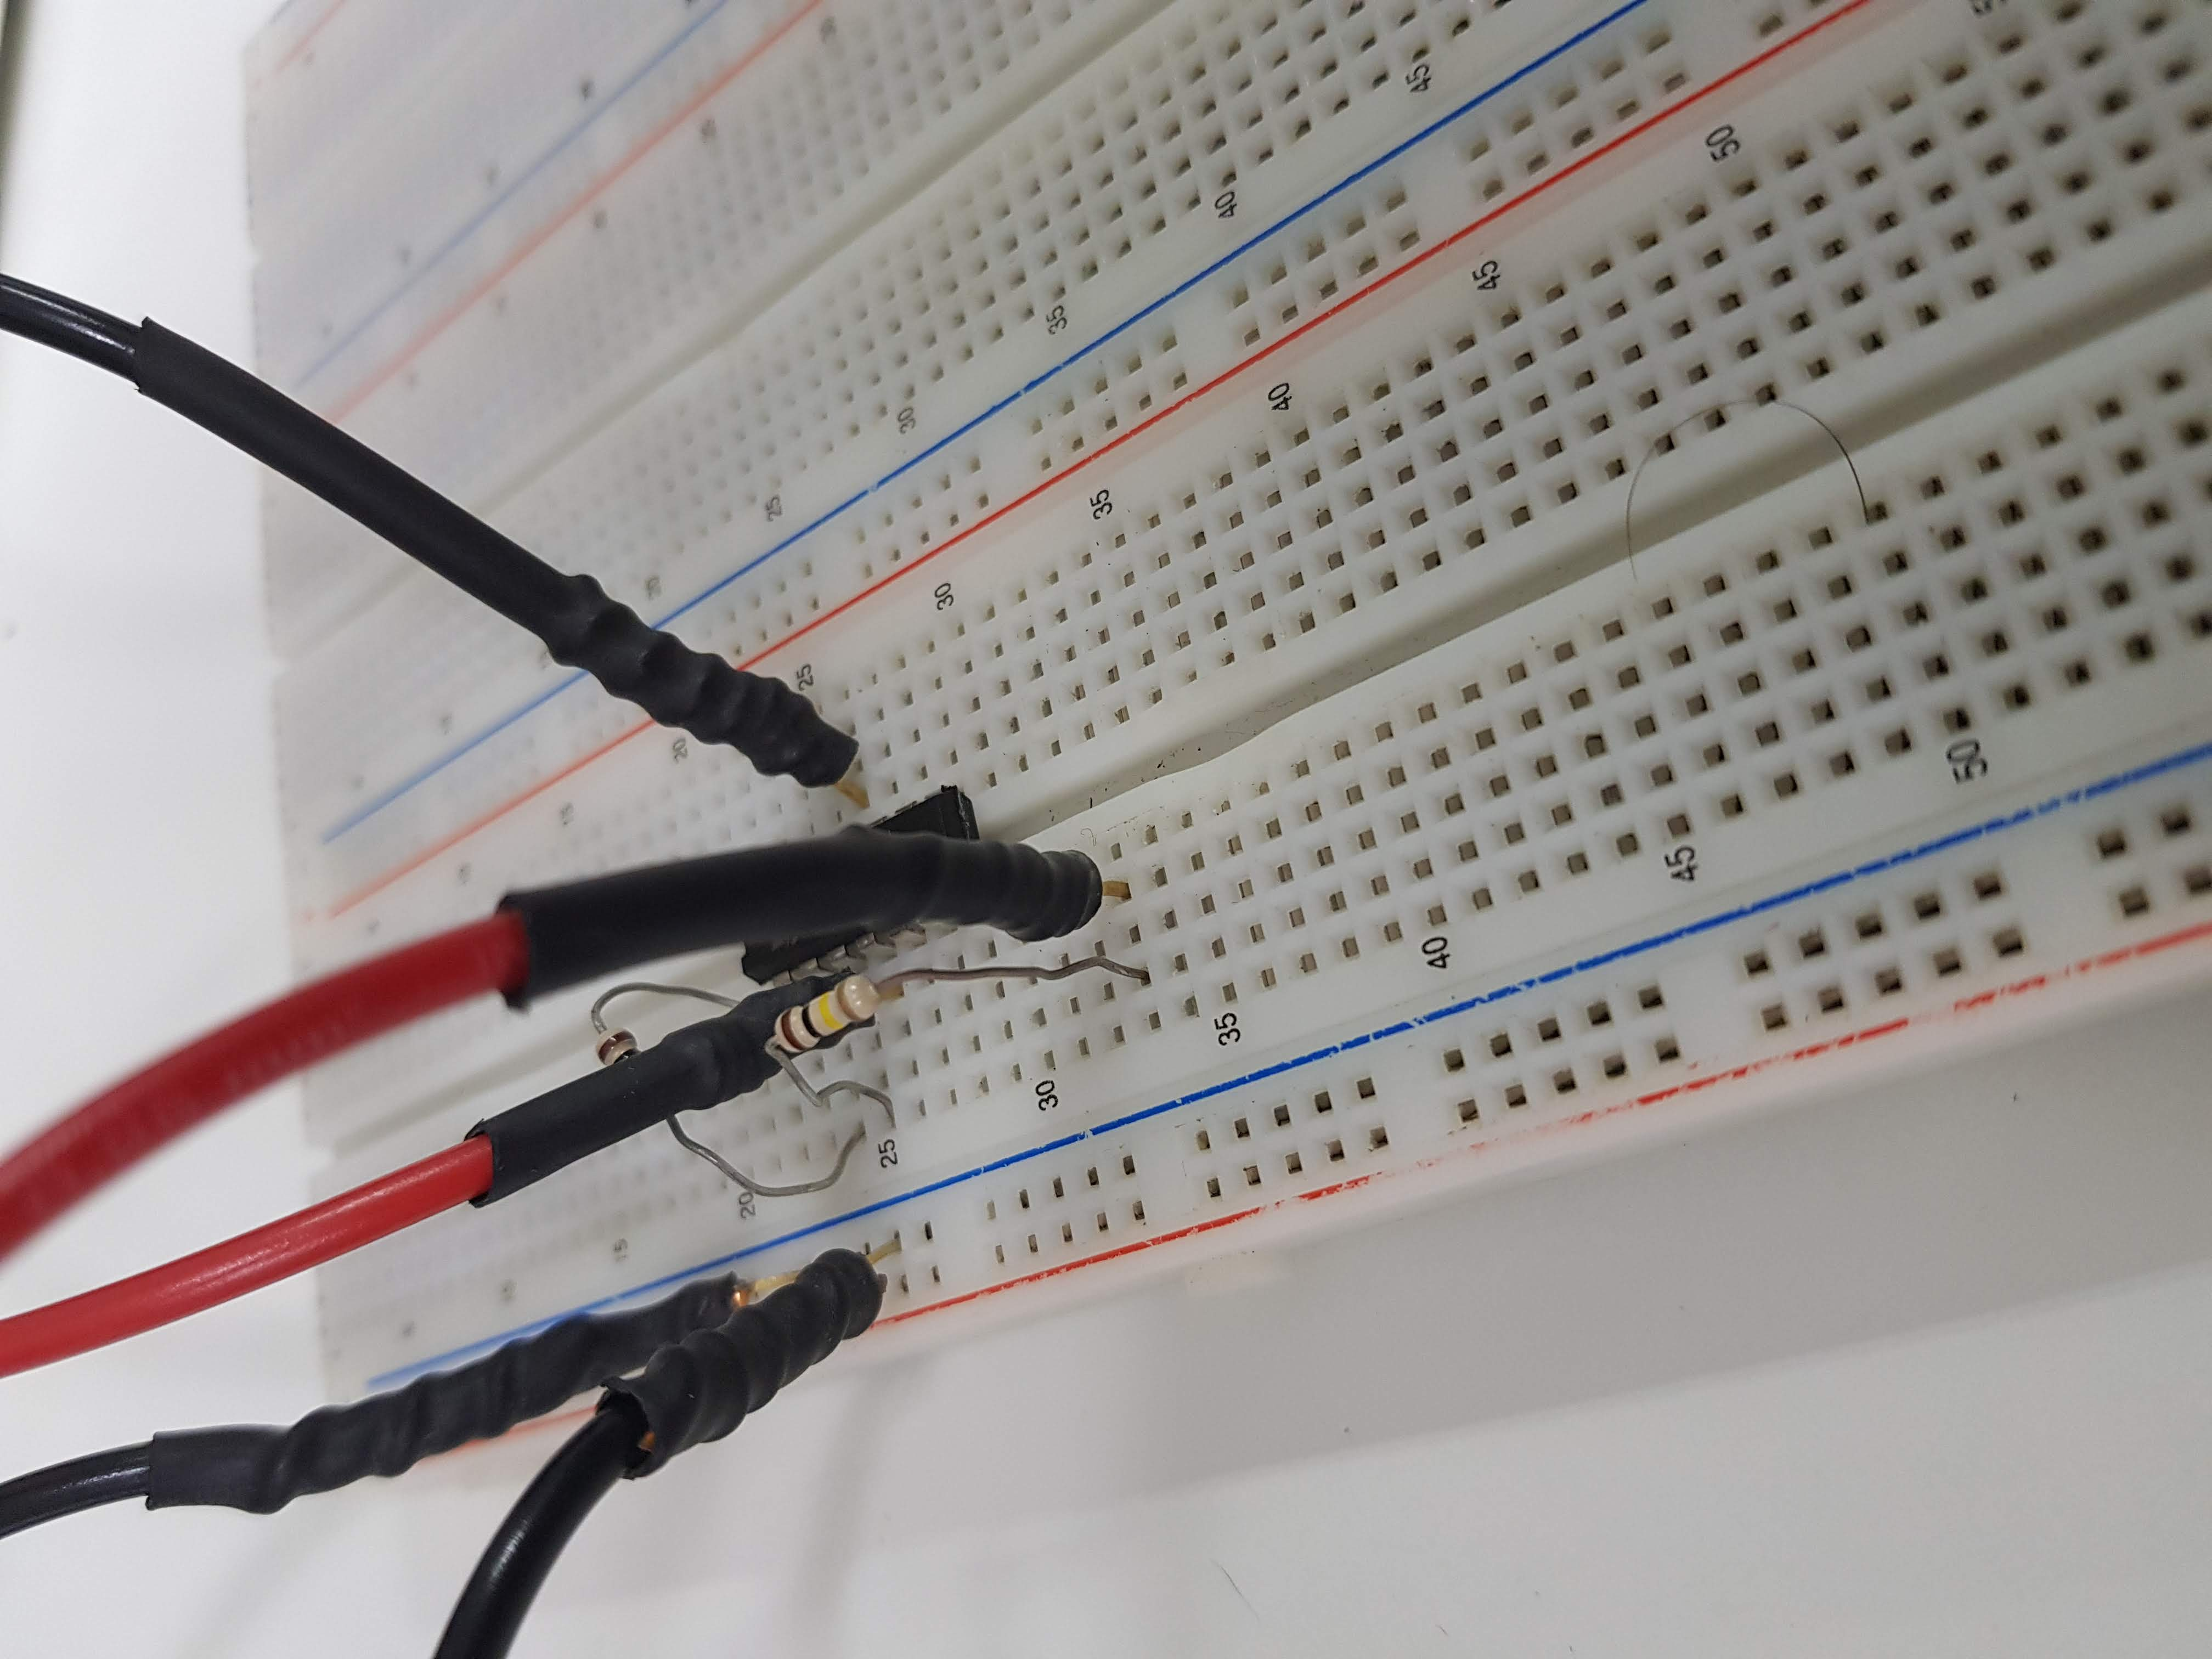
\includegraphics[scale = 0.5]{circ_3.png}
  \caption{Montagem do circuito da figura \ref{fig:circuito3} B.}
  \label{fig:montagem4}
\end{figure}

\subsubsection{Parte 2}
Para cada montagem, foram visualizadas no osciloscópio as ondas de entrada e saída, obtendo as imagens \ref{fig:inout1} e \ref{fig:inout2} para as montagens.
\begin{figure}[h]
  \centering
  \includegraphics[scale = 0.5]{new_file0.png}
  \caption{Ondas de entrada e saída para o circuito da figura \ref{fig:circuito3} A.}
  \label{fig:inout1}
\end{figure}
\begin{figure}[h]
  \centering
  \includegraphics[scale = 0.5]{new_file1.png}
  \caption{Ondas de entrada e saída para o circuito da figura \ref{fig:circuito3} B.}
  \label{fig:inout2}
\end{figure}
\subsubsection{Parte 3}

Após a aquisição dos dados necessários, foi construída a seguinte tabela:

TABELAAAAAAAAA

\subsection{Experiência 4}

Foram montados os circuitos de acordo com as figuras \ref{fig:circuito4} e \ref{fig:circuito5}, obtendo, assim, as montagens das figuras \ref{fig:montagem5} e \ref{fig:montagem6}.
Para ambas as montagens, $R_i_n = 98,3k\Omega e R_o_u_t = 98,9k\Omega$.
\begin{figure}[h]
  \centering
  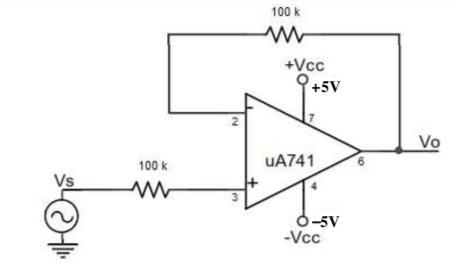
\includegraphics[scale = 0.5]{exp4-1.png}
  \caption{Medição da faixa de tensão de entrada.}
  \label{fig:circuito4}
\end{figure}
\begin{figure}[h]
  \centering
  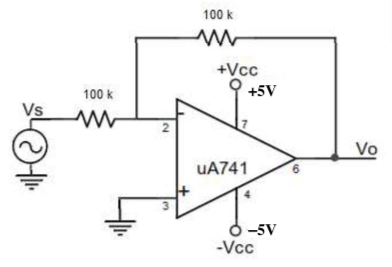
\includegraphics[scale = 0.5]{exp4-2.png}
  \caption{Medição dos intervalos de tensão de saída.}
  \label{fig:circuito5}
\end{figure}

\subsubsection{Parte 1 - Montagem}

\begin{figure}[h]
  \centering
  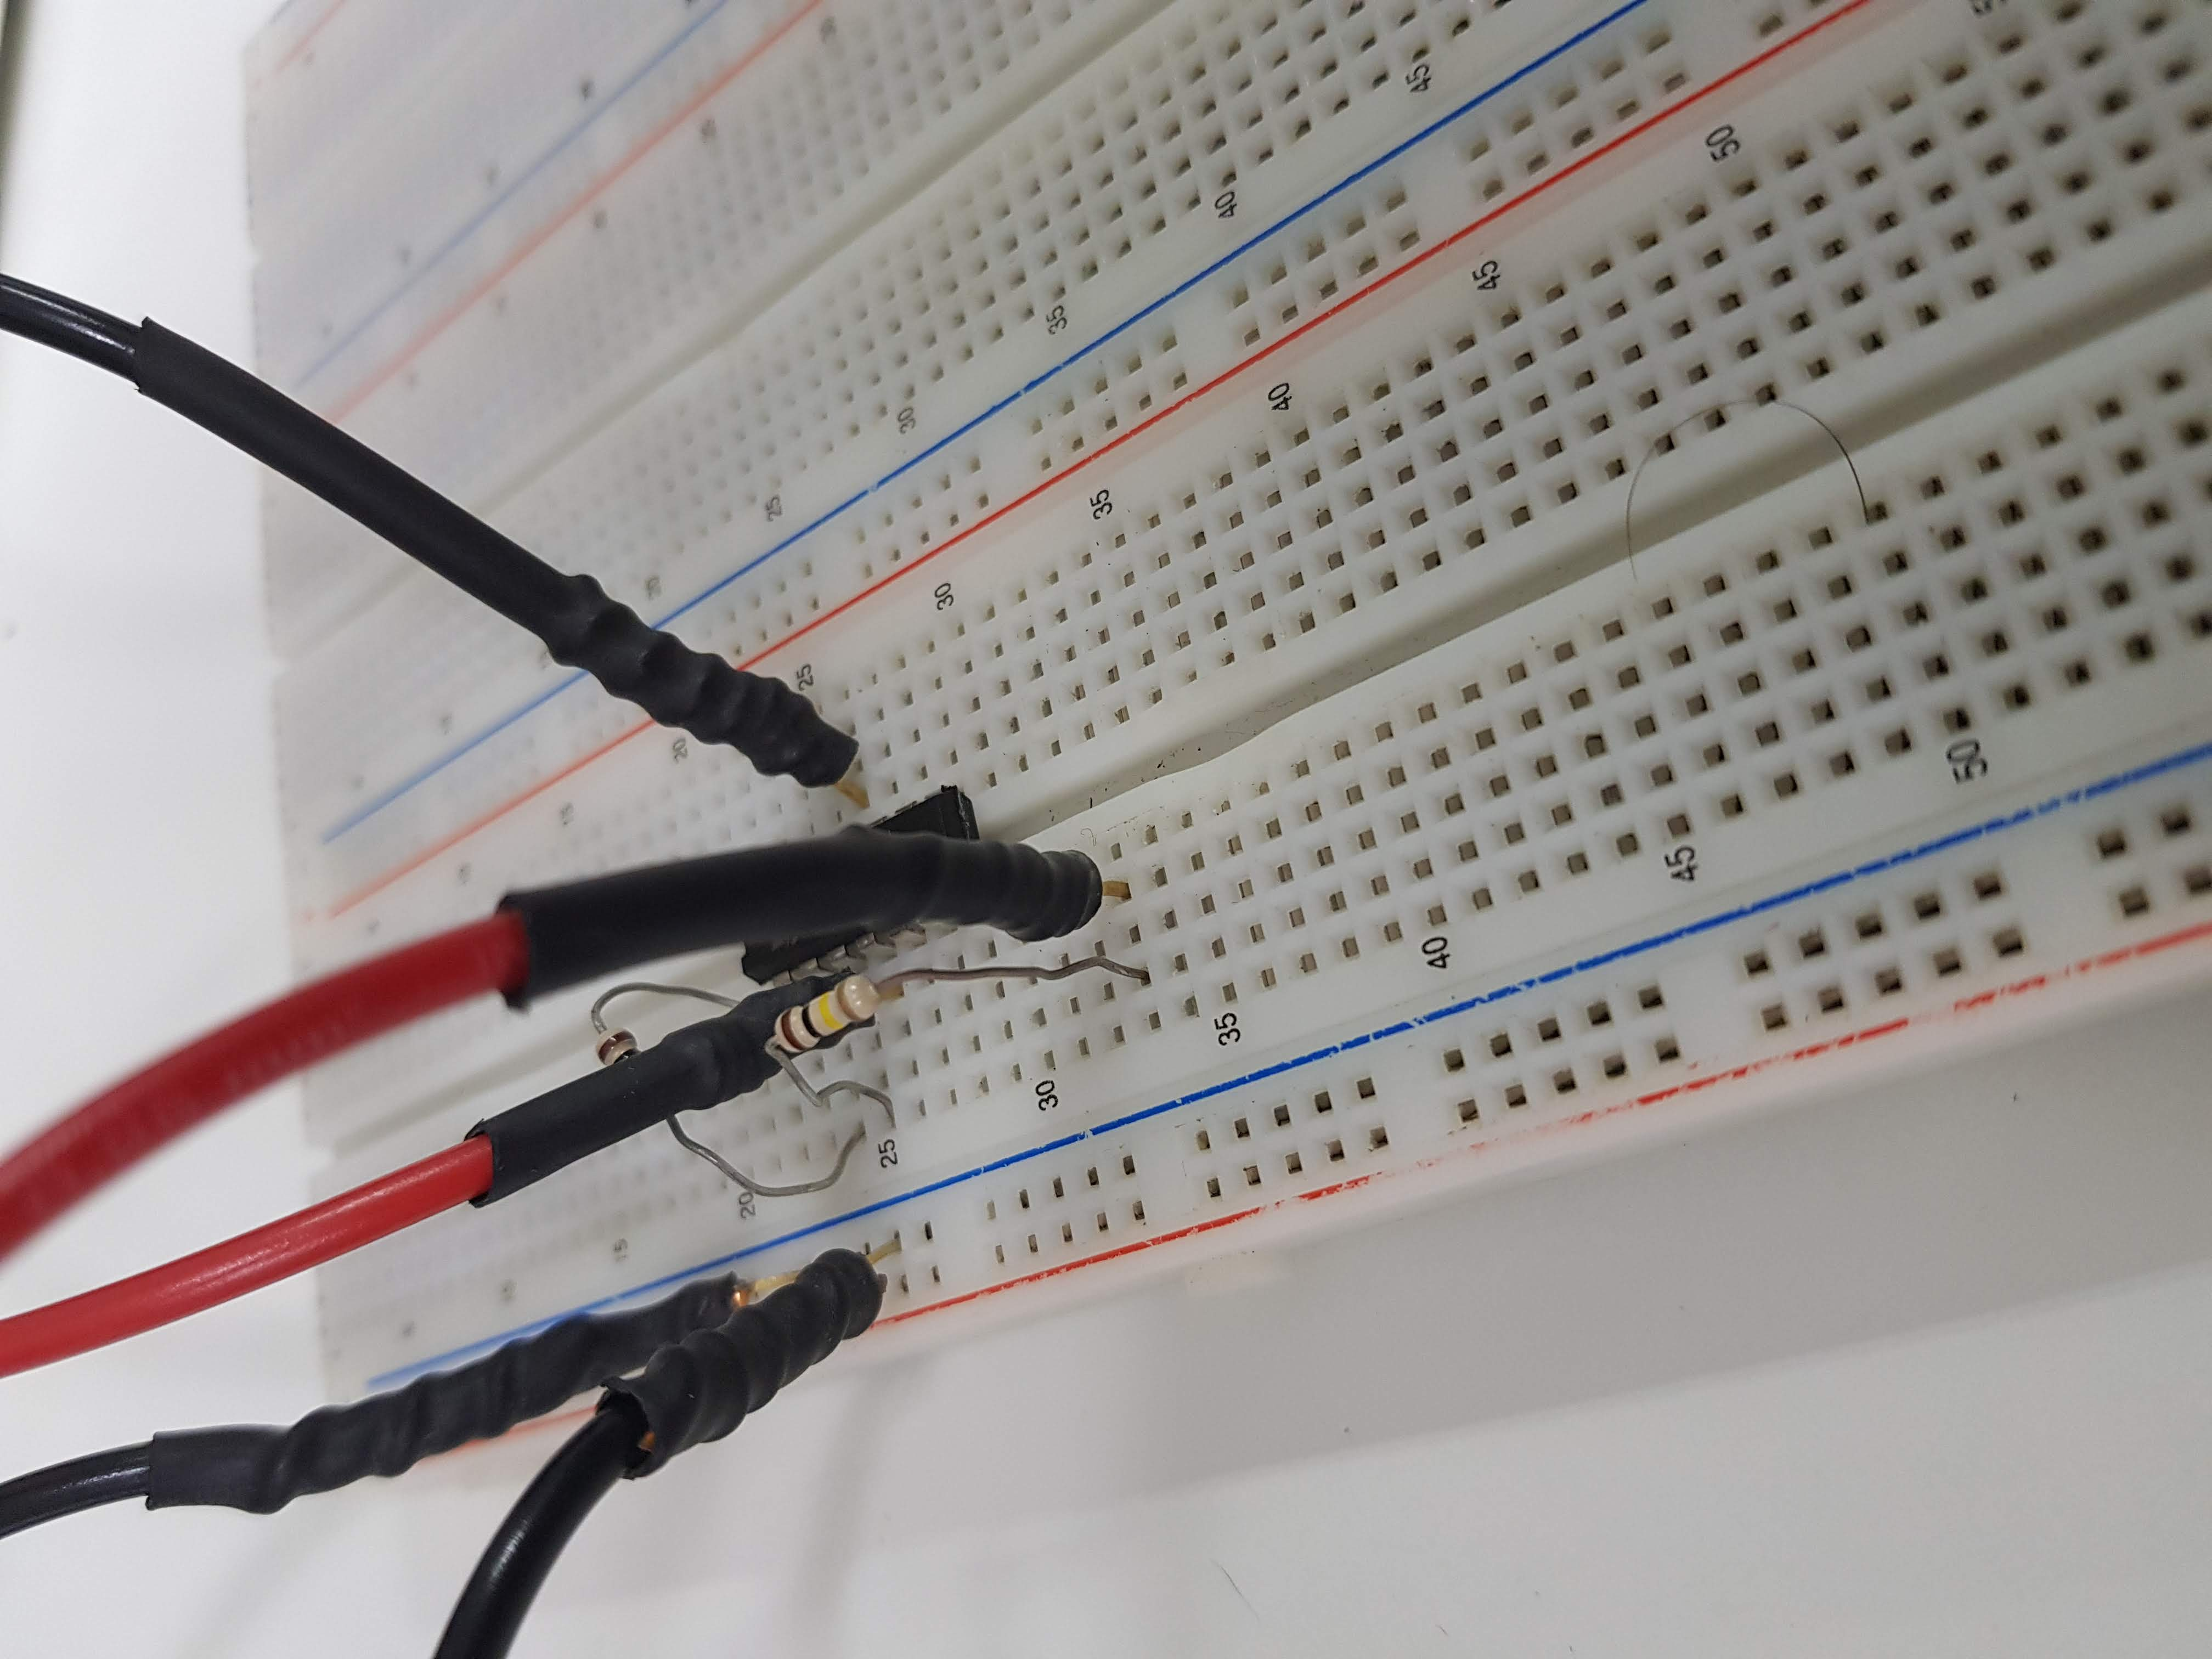
\includegraphics[scale = 0.5]{circ_3.png}
  \caption{Montagem do circuito da figura \ref{fig:circuito4}.}
  \label{fig:montagem5}
\end{figure}
\begin{figure}[h]
  \centering
  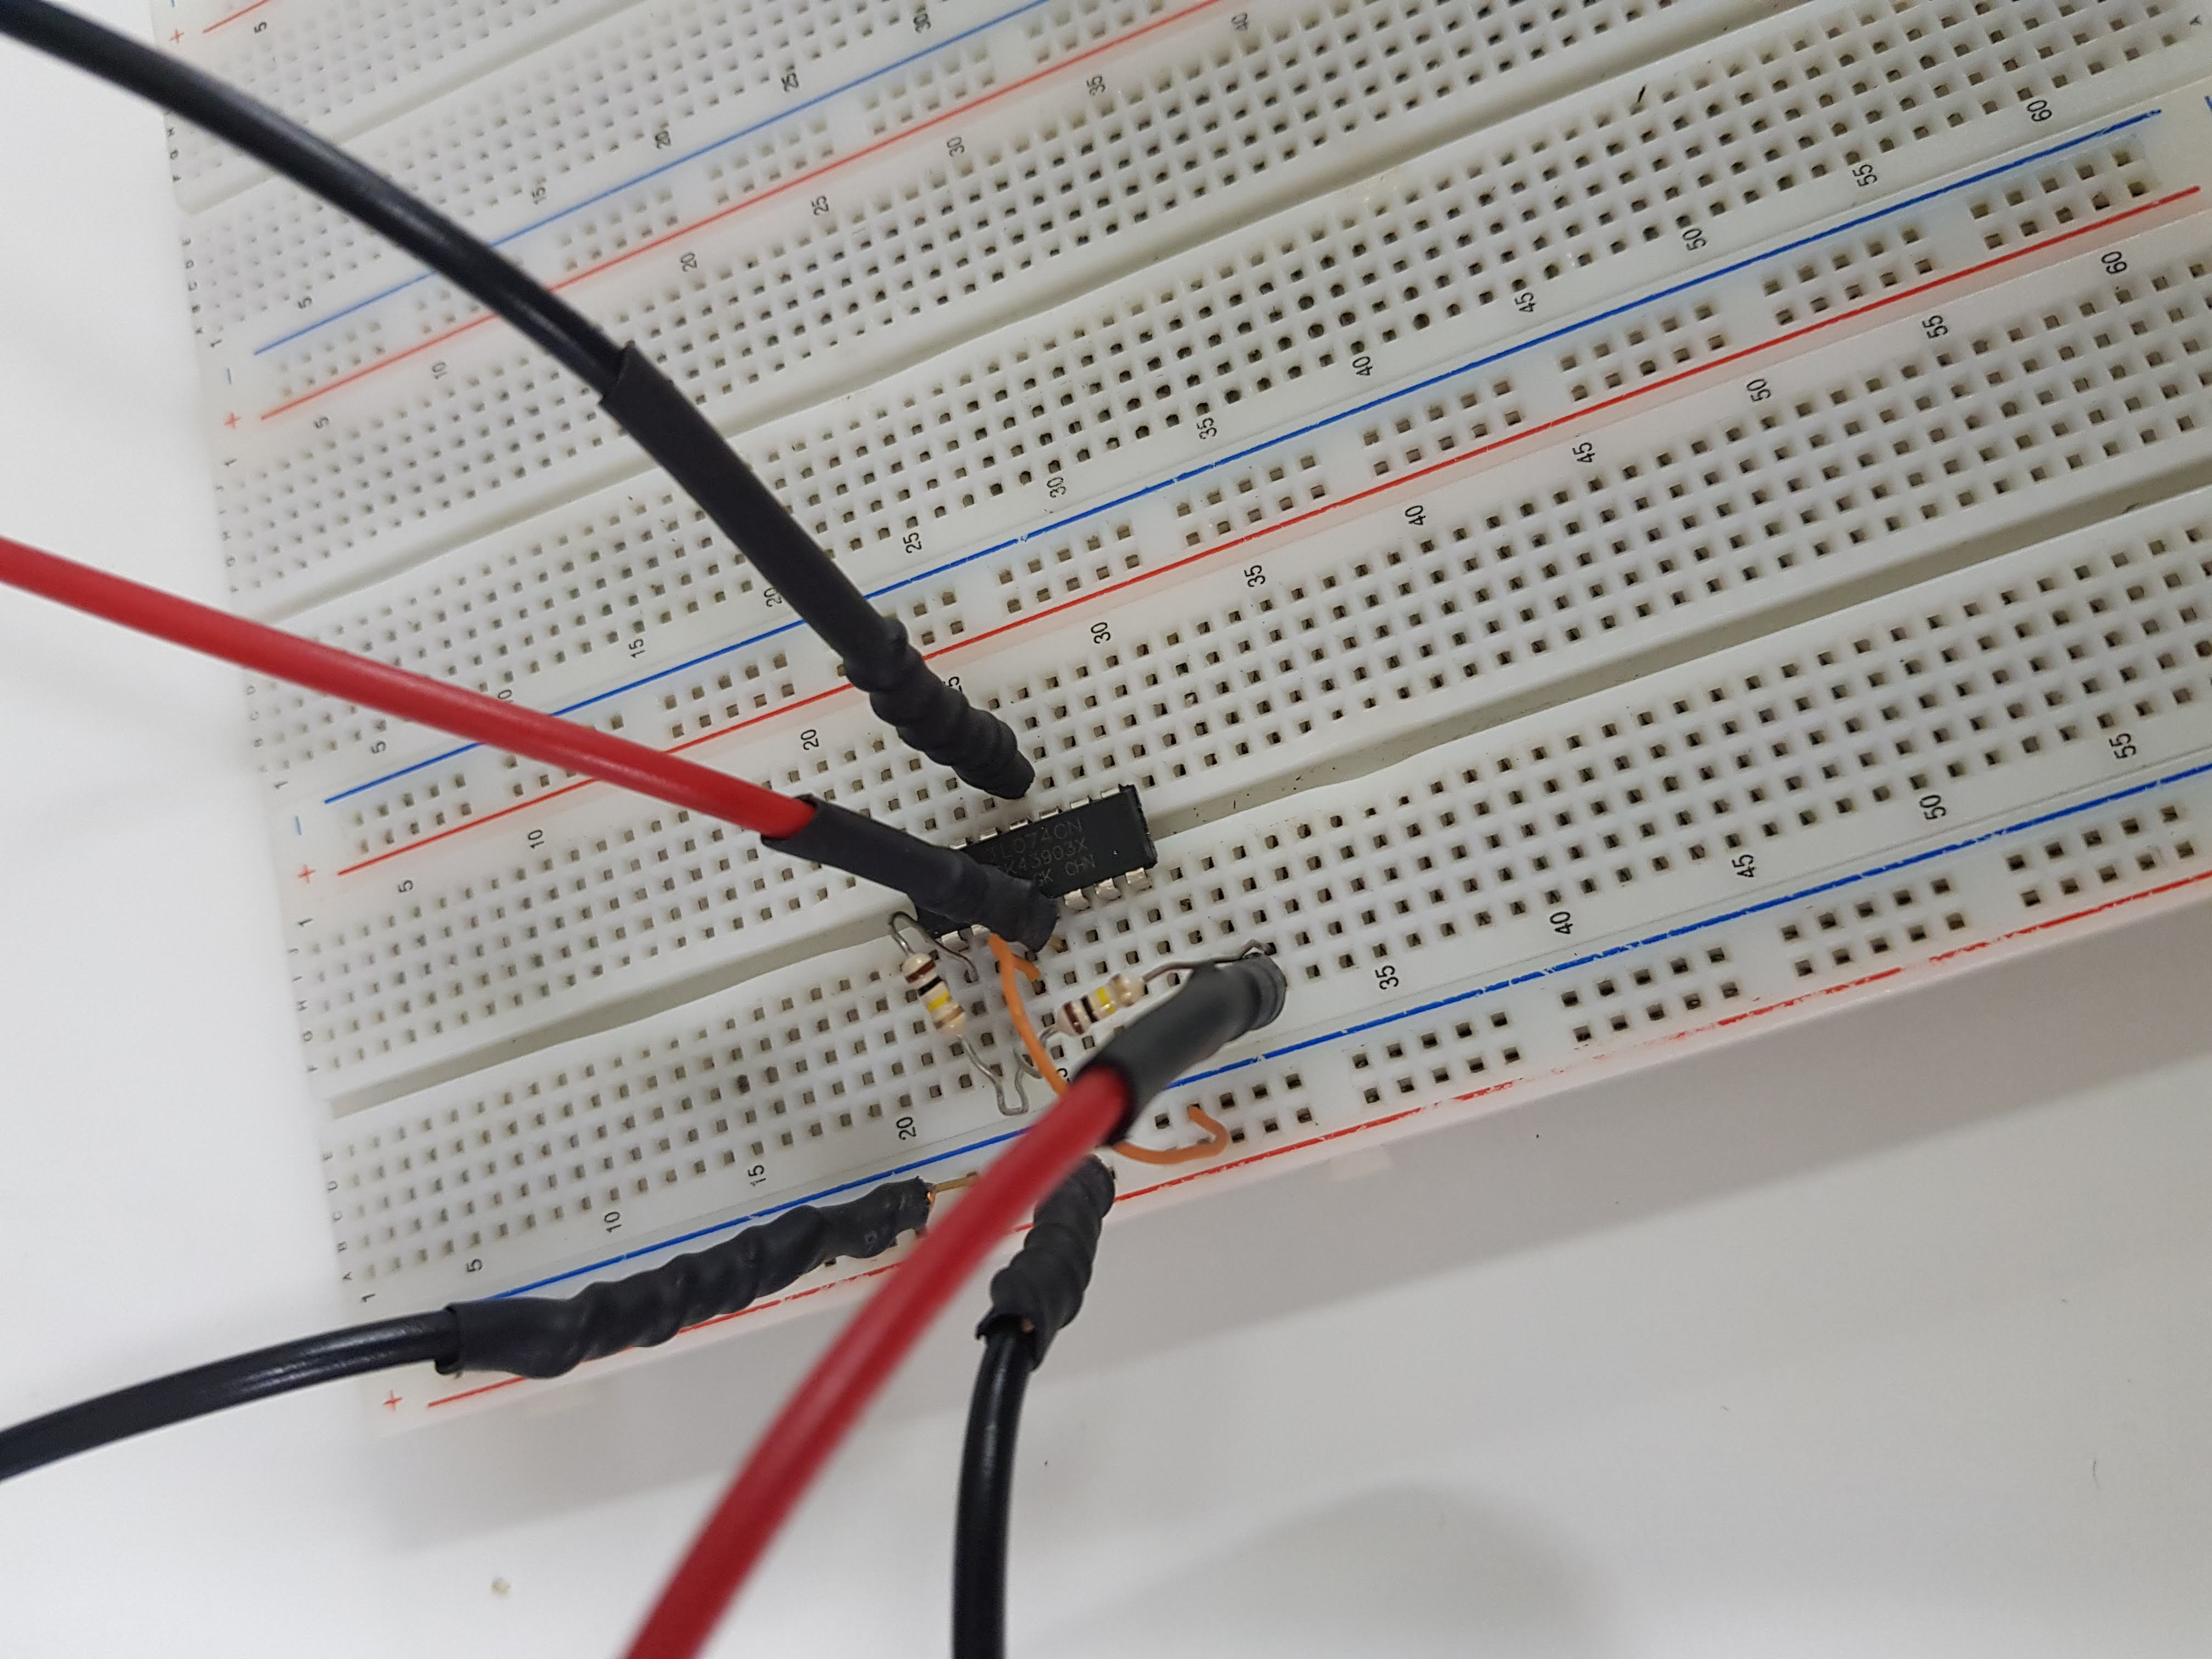
\includegraphics[scale = 0.5]{circ_4.png}
  \caption{Montagem do circuito da figura \ref{fig:circuito5}.}
  \label{fig:montagem6}
\end{figure}

\subsubsection{Parte 2}
Para a primeira montagem, foi visualizada no osciloscópio as ondas de entrada e saída, utilizando uma entrada senoidal de 5V de amplitude e 100Hz de frequência obtendo a imagen \ref{fig:inout3}.
\begin{figure}[h]
  \centering
  \includegraphics[scale = 0.5]{new_file3.png}
  \caption{Ondas de entrada e saída para o circuito da figura \ref{fig:circuito4}.}
  \label{fig:inout3}
\end{figure}

\subsubsection{Parte 3}

Foi ajustada a fonte de tensão até que não fossem observadas distorções, obtendo o resultado da imagem \ref{fig:inout4}
\begin{figure}[h]
  \centering
  \includegraphics[scale = 0.5]{new_file4.png}
  \caption{Ondas de entrada e saída para o circuito da figura \ref{fig:circuito4}.}
  \label{fig:inout4}
\end{figure}

\subsubsection{Parte 4}
Foram medidos os valores de pico positivo e negativo da tensão de entrada, obtendo

\subsubsection{Parte 5}
Foi realizado o mesmo procedimento para o circuito \ref{fig:circuito5}



\subsubsection{Parte 6}
TABELAAAAAAAAA


\chapter{Discussão}

\section{Questão 1 - Análise do circuito 1}

\subsection{parte B}

Ao aumentar a amplitude do sinal de entrada, observa-se que a amplitude do sinal de saída aumenta exponencialmente até um ponto em que o valor de pico é limitado, devido à tensão de saída se tornar maior que o limite de saturação do transistor.

Pode-se notar que ao diminuir o valor de $R_S$ houve um aumento na tensão de saída, devido ao aumento da corrente que circula no TJB, e consequentemente, em $R_L$, causando um aumento na tensão observada na saída.

É possível, então, concluir que a amplitude da componente AC é inversamente proporcional ao valor de $R_L$ devido ao fato de que a resistencia aumenta, a corrente sobre a carga diminui, diminuindo a queda de tensão em $R_L$ de modo que a tensão observada na saída é menor.

\section{Questão 2 - Análise da saída do amplificador de áudio}

O amplificador apresentou demasiada distorção do som e ruído para os metodos de teste utilizados, principalmente a música que teve sua melodia profundamente prejudicda. A baixa qualidade do som pode ter sido causada por irregularidades na membrana do microfone da caixa de som, por variações nos valores dos capacitores, pelo sinal de entrada passar do ponto de operação do amplificador ou porque o $\lambda$ dos transistores não é igual a 0.

\clearpage

\section*{Referências}

[1] SEDRA, Adel S.; SMITH, Kenneth Carless. Microelectronic circuits. New York: Oxford University Press, 1998.

[2] RAZAVI, Behzad; BEHZAD, Razavi. RF microelectronics. New Jersey: Prentice Hall, 1998.

\end{document}
